% =============================================================================
%  The assumptions of a one-dimensional PBL closure, as a pyramid -- VERTICAL version
%  GENERATED by scripts/make_pyramid_vertical.py from pbl_assumptions_pyramid.tex; edit the
%  horizontal file and regenerate. Tiers are columns (physics | concepts | formalism); a block
%  touches at its left exactly what it relies on. Scale: 0.88 cm per old cm along the ground,
%  3.0 cm per old cm of tier height. Build: tectonic pbl_assumptions_pyramid_vertical.tex
% =============================================================================
\documentclass[10pt]{article}
\usepackage{iftex}
\ifPDFTeX
  \usepackage[utf8]{inputenc}
  \usepackage[T1]{fontenc}
  \usepackage{lmodern}
\else
  \usepackage{fontspec}
  \setmainfont{lmroman10-regular.otf}[BoldFont=lmroman10-bold.otf,
    ItalicFont=lmroman10-italic.otf, BoldItalicFont=lmroman10-bolditalic.otf]
\fi
\usepackage[british]{babel}
\usepackage[a4paper,margin=10mm,top=9mm,bottom=9mm]{geometry}
\usepackage{amsmath,amssymb}
\usepackage{xcolor}
\usepackage{tikz}
\usepackage{microtype}
\pagestyle{empty}
\setlength{\parindent}{0pt}
\setlength{\parskip}{0.5ex}
% rigid math relation spacing: the centred block texts would otherwise stretch around = and <<
\thickmuskip=5mu \medmuskip=4mu \thinmuskip=3mu

% ---- notation ---------------------------------------------------------------
\newcommand{\avg}[1]{\langle #1 \rangle}
\newcommand{\pd}[2]{\partial #1/\partial #2}
\newcommand{\qsq}{q^{2}}
\newcommand{\Rfc}{R_{fc}}
\newcommand{\dx}{\Delta x}
% ---- rows the PhD concept turns on (same data as the note's macros.tex) ------
\definecolor{cKey}{HTML}{7B2D8E}
\definecolor{cGXIX}{HTML}{990011}   % Goger 2019 port (the note's colour)
\definecolor{cFULL}{HTML}{7B2D8E}   % Kosovic-Juliano 3D closure (the note's colour)
% \hl{x0}{x1}{y0}{y1}{colour}{inset}: a frame inside a block, marking a scheme's decisive block
\newcommand{\hl}[6]{\draw[#5, line width=1.1pt] (#1+#6,#3+#6) rectangle (#2-#6,#4-#6);}
\newcommand{\setkey}[2]{\expandafter\def\csname key@#1\endcsname{#2}}
\makeatletter
\setkey{A1}{1}\setkey{B1}{1}\setkey{B2}{1}\setkey{B3}{1}\setkey{C3}{1}\setkey{C4}{1}\setkey{C6}{1}\setkey{C7}{1}
\setkey{B5}{2}\setkey{B6}{2}\setkey{C2}{2}\setkey{C5}{2}\setkey{C9}{2}
\newcommand{\keymark}[1]{\ifcsname key@#1\endcsname
  \if1\csname key@#1\endcsname\textcolor{cKey}{$\blacktriangleright$}\else\textcolor{cKey}{$\triangleright$}\fi\fi}
\makeatother
\newcommand{\pid}[1]{\keymark{#1}\textbf{#1}}
% \pb{x0}{x1}{y0}{y1}{style}{text}: a block from (x0,y0) to (x1,y1), text centred
\newcommand{\pbf}[7]{\pgfmathsetmacro{\pbw}{#2-#1-#7}%
  \draw[#5] (#1,#3) rectangle (#2,#4);
  \node[align=center, font=\tiny, inner sep=0pt, text width=\pbw cm] at ({(#1+#2)/2},{(#3+#4)/2}) {#6};}
\newcommand{\pb}[6]{\pgfmathsetmacro{\pbw}{#2-#1-0.20}%
  \draw[#5] (#1,#3) rectangle (#2,#4);
  \node[align=center, font=\tiny, inner sep=0pt, text width=\pbw cm] at ({(#1+#2)/2},{(#3+#4)/2}) {#6};}


% vertical block: rectangle + centred text, text width = block width - hpad
\newcommand{\pbv}[7]{\pgfmathsetmacro{\pbw}{#2-#1-#7}%
  \draw[#5] (#1,#3) rectangle (#2,#4);
  \node[align=center, font=\scriptsize, inner sep=0pt, text width=\pbw cm] at ({(#1+#2)/2},{(#3+#4)/2}) {#6};}
\newcommand{\hlv}[6]{\draw[#5, line width=1.1pt] (#1+#6,#3+#6) rectangle (#2-#6,#4-#6);}

\begin{document}
{\large\bfseries The assumptions of a one-dimensional PBL closure, as a pyramid: what rests on what}\\[0.2ex]
{\small Vertical version of the companion page to the assumptions note. 2026-09-16.}

\vspace{0.3ex}
{\footnotesize Left column, dark grey: the physical hypotheses. Middle, light grey: the concepts of turbulence theory
that follow from them. Right, white: the formal statements of the level-2.5 closure. A block touches at its left
exactly the blocks it relies on; blocks in one column do not touch. Frames: \textcolor{cGXIX}{\textbf{red}} the Goger
2019 port, \textcolor{cFULL}{\textbf{purple}} the Kosovi\'c--Juliano three-dimensional closure, nested both. The
rules, the reading and the correspondence to the note's rows are on the next page.\par}

\vspace{0.4ex}
\begin{center}
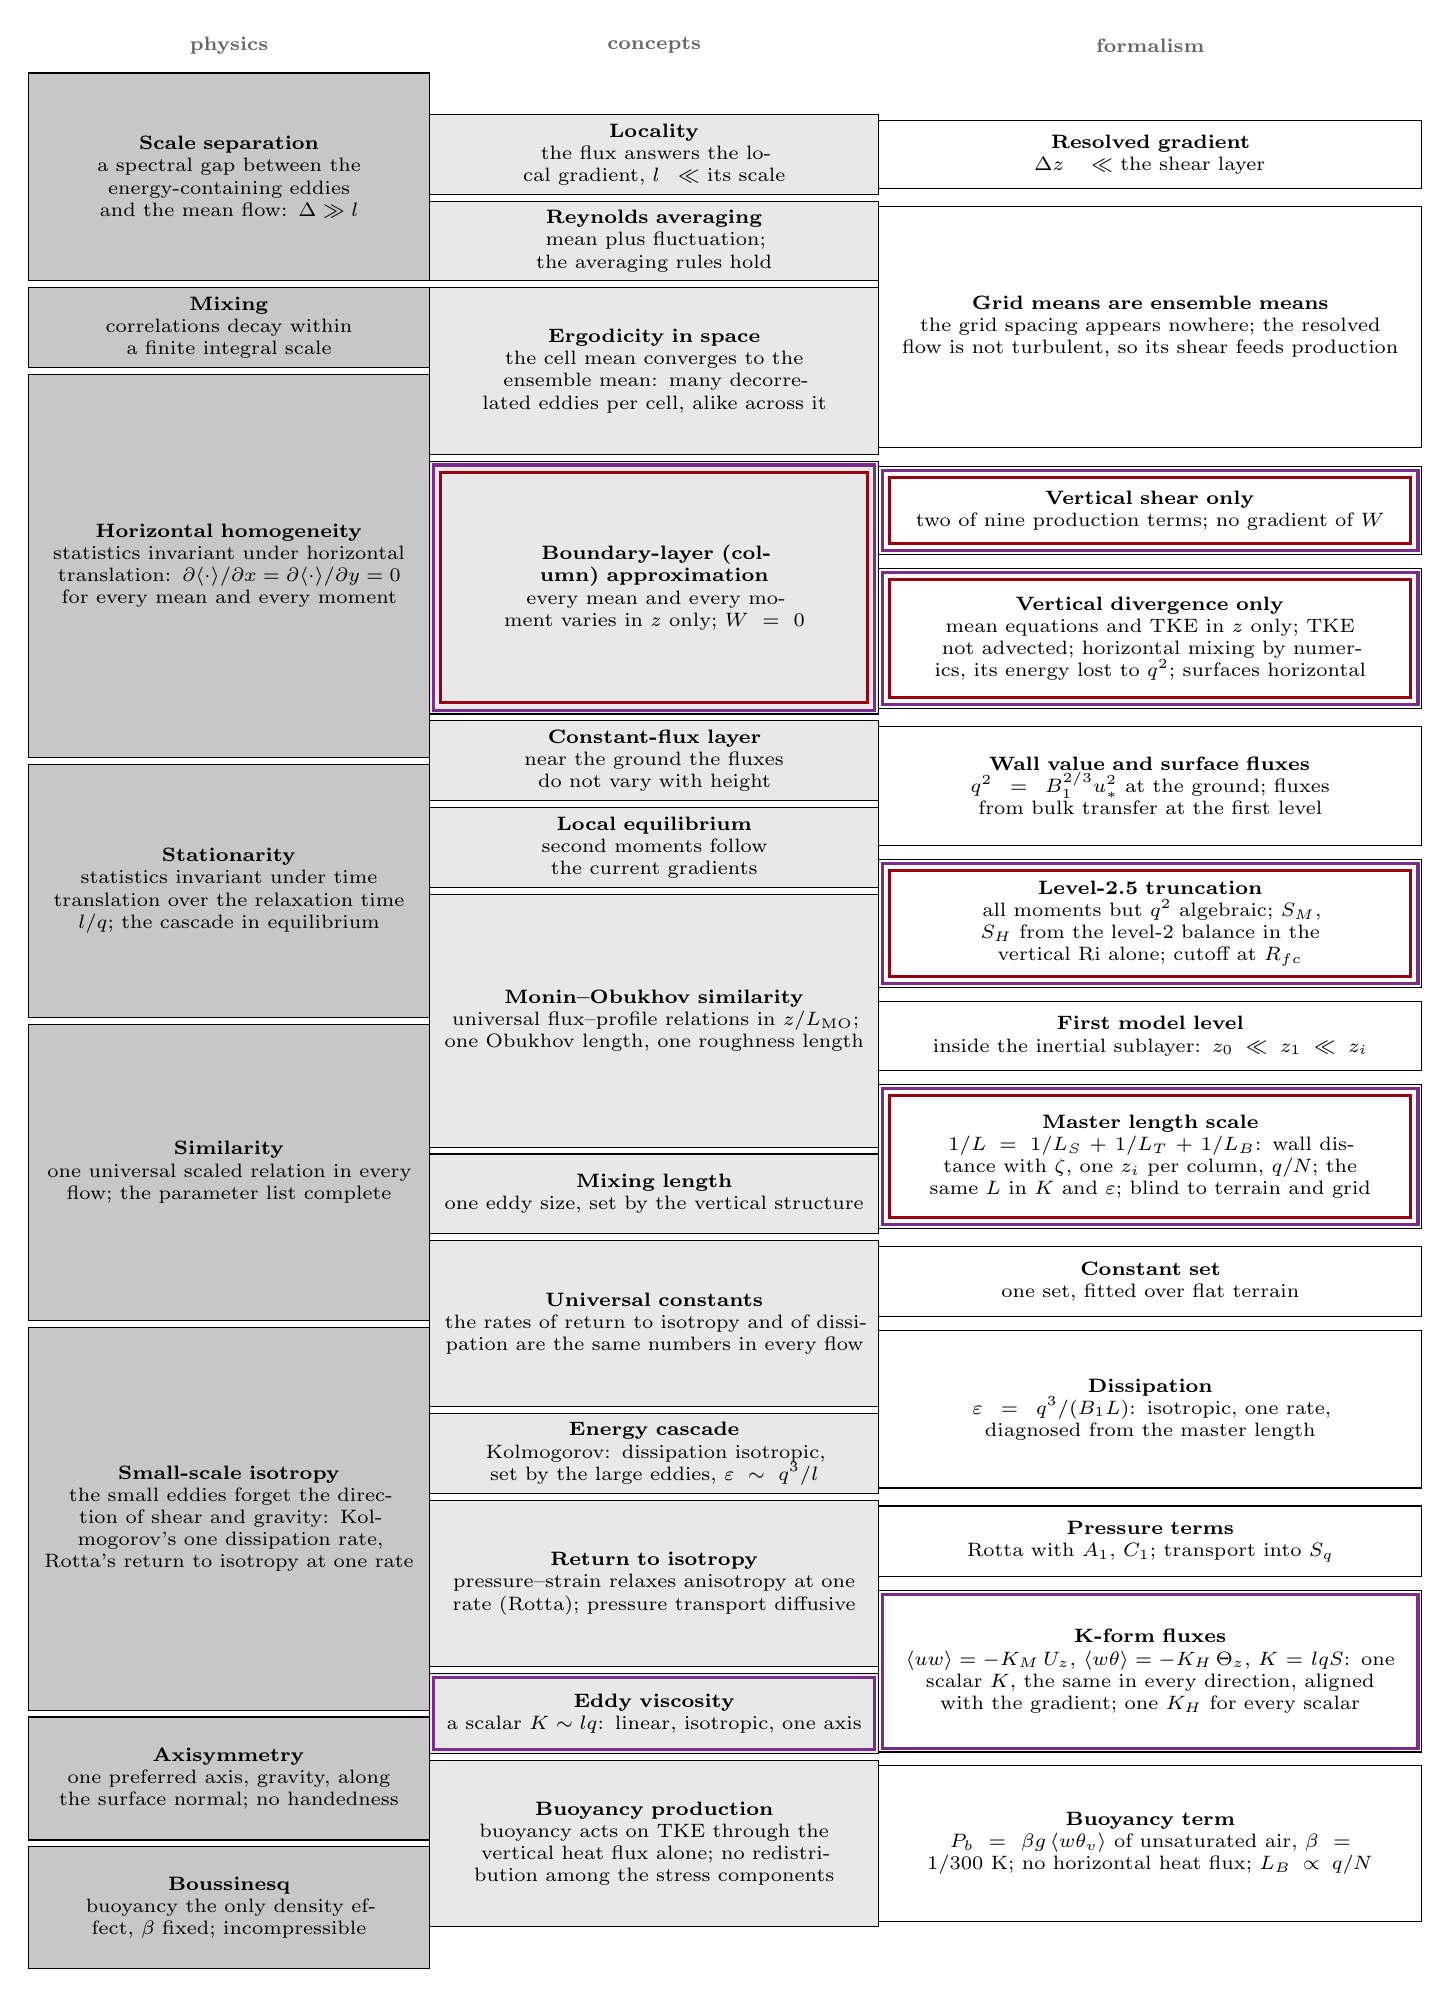
\begin{tikzpicture}[x=1cm, y=1cm,
  ground/.style={draw, line width=0.4pt, fill=black!22},
  hyp/.style={draw, line width=0.4pt, fill=black!9},
  row/.style={draw, line width=0.4pt, fill=white}]
\node[font=\scriptsize\bfseries, text=black!60] at (2.550,24.418) {physics};
\node[font=\scriptsize\bfseries, text=black!60] at (7.950,24.418) {concepts};
\node[font=\scriptsize\bfseries, text=black!60] at (14.250,24.418) {formalism};
\pbv{0.000}{5.100}{21.428}{24.068}{ground}{\textbf{Scale separation}\\ a spectral gap between the energy-containing eddies and the mean flow: \mbox{$\Delta \gg l$}}{0.30}
\pbv{0.000}{5.100}{20.328}{21.340}{ground}{\textbf{Mixing}\\ correlations decay within a finite integral scale}{0.30}
\pbv{0.000}{5.100}{15.378}{20.240}{ground}{\textbf{Horizontal homogeneity}\\ statistics invariant under horizontal translation: \mbox{$\pd{\avg{\cdot}}{x} = \pd{\avg{\cdot}}{y} = 0$} for every mean and every moment}{0.30}
\pbv{0.000}{5.100}{12.078}{15.290}{ground}{\textbf{Stationarity}\\ statistics invariant under time translation over the relaxation time $l/q$; the cascade in equilibrium}{0.30}
\pbv{0.000}{5.100}{8.228}{11.990}{ground}{\textbf{Similarity}\\ one universal scaled relation in every flow; the parameter list complete}{0.30}
\pbv{0.000}{5.100}{3.278}{8.140}{ground}{\textbf{Small-scale isotropy}\\ the small eddies forget the direction of shear and gravity: Kolmogorov's one dissipation rate, Rotta's return to isotropy at one rate}{0.30}
\pbv{0.000}{5.100}{1.628}{3.190}{ground}{\textbf{Axisymmetry}\\ one preferred axis, gravity, along the surface normal; no handedness}{0.30}
\pbv{0.000}{5.100}{0.000}{1.540}{ground}{\textbf{Boussinesq}\\ buoyancy the only density effect, $\beta$ fixed; incompressible}{0.30}
\pbv{5.100}{10.800}{22.528}{23.540}{hyp}{\textbf{Locality}\\ the flux answers the local gradient, $l \ll$ its scale}{0.30}
\pbv{5.100}{10.800}{21.428}{22.440}{hyp}{\textbf{Reynolds averaging}\\ mean plus fluctuation; the averaging rules hold}{0.30}
\pbv{5.100}{10.800}{19.228}{21.340}{hyp}{\textbf{Ergodicity in space}\\ the cell mean converges to the ensemble mean: many decorrelated eddies per cell, alike across it}{0.30}
\pbv{5.100}{10.800}{15.928}{19.140}{hyp}{\textbf{Boundary-layer (column) approximation}\\ every mean and every moment varies in $z$ only; $W = 0$}{0.56}
\pbv{5.100}{10.800}{14.828}{15.840}{hyp}{\textbf{Constant-flux layer}\\ near the ground the fluxes do not vary with height}{0.30}
\pbv{5.100}{10.800}{13.728}{14.740}{hyp}{\textbf{Local equilibrium}\\ second moments follow the current gradients}{0.30}
\pbv{5.100}{10.800}{10.428}{13.640}{hyp}{\textbf{Monin--Obukhov similarity}\\ universal flux--profile relations in $z/L_{\mathrm{MO}}$; one Obukhov length, one roughness length}{0.30}
\pbv{5.100}{10.800}{9.328}{10.340}{hyp}{\textbf{Mixing length}\\ one eddy size, set by the vertical structure}{0.30}
\pbv{5.100}{10.800}{7.128}{9.240}{hyp}{\textbf{Universal constants}\\ the rates of return to isotropy and of dissipation are the same numbers in every flow}{0.30}
\pbv{5.100}{10.800}{6.028}{7.040}{hyp}{\textbf{Energy cascade}\\ Kolmogorov: dissipation isotropic, set by the large eddies, $\varepsilon \sim q^3/l$}{0.30}
\pbv{5.100}{10.800}{3.828}{5.940}{hyp}{\textbf{Return to isotropy}\\ pressure--strain relaxes anisotropy at one rate (Rotta); pressure transport diffusive}{0.30}
\pbv{5.100}{10.800}{2.728}{3.740}{hyp}{\textbf{Eddy viscosity}\\ a scalar $K \sim l q$: linear, isotropic, one axis}{0.40}
\pbv{5.100}{10.800}{0.528}{2.640}{hyp}{\textbf{Buoyancy production}\\ buoyancy acts on TKE through the vertical heat flux alone; no redistribution among the stress components}{0.30}
\pbv{10.800}{17.700}{22.598}{23.470}{row}{\textbf{Resolved gradient}\\ $\Delta z \ll$ the shear layer}{0.30}
\pbv{10.800}{17.700}{19.316}{22.370}{row}{\textbf{Grid means are ensemble means}\\ the grid spacing appears nowhere; the resolved flow is not turbulent, so its shear feeds production}{0.30}
\pbv{10.800}{17.700}{17.952}{19.070}{row}{\textbf{Vertical shear only}\\ two of nine production terms; no gradient of $W$}{0.56}
\pbv{10.800}{17.700}{15.998}{17.776}{row}{\textbf{Vertical divergence only}\\ mean equations and TKE in $z$ only; TKE not advected; horizontal mixing by numerics, its energy lost to $\qsq$; surfaces horizontal}{0.56}
\pbv{10.800}{17.700}{14.256}{15.770}{row}{\textbf{Wall value and surface fluxes}\\ $\qsq = B_1^{2/3} u_*^2$ at the ground; fluxes from bulk transfer at the first level}{0.30}
\pbv{10.800}{17.700}{12.452}{14.080}{row}{\textbf{Level-2.5 truncation}\\ all moments but $\qsq$ algebraic; $S_M$, $S_H$ from the level-2 balance in the vertical Ri alone; cutoff at $\Rfc$}{0.56}
\pbv{10.800}{17.700}{11.396}{12.276}{row}{\textbf{First model level}\\ inside the inertial sublayer: $z_0 \ll z_1 \ll z_i$}{0.30}
\pbv{10.800}{17.700}{9.398}{11.220}{row}{\textbf{Master length scale}\\ $1/L = 1/L_S + 1/L_T + 1/L_B$: wall distance with $\zeta$, one $z_i$ per column, $q/N$; the same $L$ in $K$ and $\varepsilon$; blind to terrain and grid}{0.56}
\pbv{10.800}{17.700}{8.272}{9.170}{row}{\textbf{Constant set}\\ one set, fitted over flat terrain}{0.30}
\pbv{10.800}{17.700}{6.098}{8.096}{row}{\textbf{Dissipation}\\ $\varepsilon = q^3/(B_1 L)$: isotropic, one rate, diagnosed from the master length}{0.30}
\pbv{10.800}{17.700}{4.972}{5.870}{row}{\textbf{Pressure terms}\\ Rotta with $A_1$, $C_1$; transport into $S_q$}{0.30}
\pbv{10.800}{17.700}{2.746}{4.796}{row}{\textbf{K-form fluxes}\\ \mbox{$\avg{uw} = -K_M\,U_z$}, \mbox{$\avg{w\theta} = -K_H\,\Theta_z$}, $K = l q S$: one scalar $K$, the same in every direction, aligned with the gradient; one $K_H$ for every scalar}{0.40}
\pbv{10.800}{17.700}{0.598}{2.570}{row}{\textbf{Buoyancy term}\\ $P_b = \beta g\,\avg{w\theta_v}$ of unsaturated air, $\beta = 1/300$~K; no horizontal heat flux; $L_B \propto q/N$}{0.30}
\hlv{5.100}{10.800}{15.928}{19.140}{cFULL}{0.05}
\hlv{5.100}{10.800}{15.928}{19.140}{cGXIX}{0.14}
\hlv{10.800}{17.700}{17.952}{19.070}{cFULL}{0.05}
\hlv{10.800}{17.700}{17.952}{19.070}{cGXIX}{0.14}
\hlv{10.800}{17.700}{15.998}{17.776}{cFULL}{0.05}
\hlv{10.800}{17.700}{15.998}{17.776}{cGXIX}{0.14}
\hlv{10.800}{17.700}{12.452}{14.080}{cFULL}{0.05}
\hlv{10.800}{17.700}{12.452}{14.080}{cGXIX}{0.14}
\hlv{10.800}{17.700}{9.398}{11.220}{cFULL}{0.05}
\hlv{10.800}{17.700}{9.398}{11.220}{cGXIX}{0.14}
\hlv{5.100}{10.800}{2.728}{3.740}{cFULL}{0.05}
\hlv{10.800}{17.700}{2.746}{4.796}{cFULL}{0.05}
\end{tikzpicture}
\end{center}

\newpage
{\footnotesize Every block is an assumption a boundary-layer scheme makes in order to run. A block touches at its
left exactly the blocks it relies on, and blocks in one column do not touch each other. Three columns. Dark grey,
the ground (left column): eight hypotheses about the fluid and the flow that rest on nothing else here. Light grey, the
concepts (middle column): the constructs of turbulence theory that follow from the ground and that every closure of this family
speaks in --- Reynolds averaging, the column approximation, the constant-flux layer, Monin--Obukhov similarity,
the mixing length, the eddy viscosity, Rotta's return to isotropy, Kolmogorov's cascade. White, the formalism (right column):
the statements of the level-2.5 closure as written, each resting on the concepts it applies. Each block shows its
primary reliance; the incidence matrix of the note has the full set. Not drawn, because no scheme needs them to
run: ergodicity in time and Taylor's hypothesis, which carry the observations and the calibration; the
constraints realizability and Galilean invariance, which bound the algebra rather than carry a block; and the
dynamical core's numerical dissipation.\par}


\vspace{0.6ex}
{\footnotesize\textbf{Frames.} The blocks each scheme's design turns on, the framed cells of the note's Table~I.0,
in the note's scheme colours. \textcolor{cGXIX}{\textbf{Red}}, the Goger 2019 port: it adds a horizontal
shear-production source to the TKE budget (vertical shear only), pays it with the energy the numerical
horizontal operator would otherwise lose and advects TKE (vertical divergence only), gives the source its own
horizontal length from the flow, $l_h^2 = U^2 T_{L,u} T_{L,v}$ (master length scale), and adds a source that knows no
Richardson number to a scheme that keeps the cutoff (level-2.5 truncation); at the concept level it breaks the
column approximation for production alone and keeps every other block. \textcolor{cFULL}{\textbf{Purple}}, the
Kosovi\'c--Juliano three-dimensional closure: it drops the column approximation entirely --- nine production
terms, three-dimensional divergences and TKE transport, metric-corrected gradients, all subgrid mixing from the
closure --- and replaces the eddy viscosity and the K-form by the solved algebraic stress tensor, so no $K$, no
alignment, no stability functions and no cutoff; the equilibrium follows from the full strain. It keeps the master
length scale, one scalar $l$ for the whole tensor: the last one-dimensional block in a three-dimensional scheme, and
the frontier. Nested frames: both schemes; every block the Goger port touches, the three-dimensional closure touches
too, and it alone reaches the eddy viscosity and the K-form.\par}

\vspace{0.4ex}
{\footnotesize\textbf{Reading.} The ground is the physics; nothing in it names a model. The middle column is where
the model's vocabulary is born: scale separation gives Reynolds averaging and locality; mixing with homogeneity gives ergodicity in space; homogeneity gives the
column approximation and, with stationarity, the constant-flux layer; stationarity gives local equilibrium and,
with similarity, Monin--Obukhov similarity; similarity gives the mixing length and, with small-scale isotropy,
universal constants; small-scale isotropy gives the cascade, the return to isotropy and, with one axis, a scalar
eddy viscosity; one axis and a Boussinesq fluid give buoyancy production through the vertical heat flux. The right
column is the closure as written, and every one of its statements applies one or two concepts: the truncation
applies local equilibrium and takes its stability functions from the surface-layer relations they were fitted
to; the master length takes its wall branch from Monin--Obukhov similarity and its shape from the mixing length;
the dissipation takes its form from the cascade and its constant from universality; the K-form takes its scalar
from the eddy viscosity and its coefficients from the return to isotropy. Terrain breaks the ground at the top
and in the middle --- homogeneity, the column, the constant-flux layer, one axis --- and the grey zone breaks it
at the very top; the lower third, isotropy and its constants, is the part no scheme in the comparison touches.\par}

\vspace{0.5ex}
{\footnotesize\textbf{Correspondence to the note's rows.} Grid means are ensemble means: A1, A2. Vertical shear only: B1, B2. Vertical divergence only: B3, B4, B5, B7. Constant-flux layer with Monin--Obukhov similarity:
B6, split because one block cannot touch three foundations. Wall value and surface fluxes: the lower boundary of
the TKE equation (D6). First model level: D3. Resolved gradient: D4. K-form fluxes: C1, C2, C3 and the mixing of
all scalars alike. Master length scale: C4 with the one-length statement of C5. Dissipation: C5. Level-2.5
truncation: C6, C7. Buoyancy term: C8 with the dry buoyancy flux (D5). Constant set: C9. Pressure terms: C10.
Which scheme drops which statement is Table~I.0 of the note.\par}

\end{document}
